% Research poster: Bredesen Center / University of Tennessee, Knoxville
% 48 x 32 in, three columns. Compile with: latexmk -pdf main.tex
\documentclass{article}

% ---------- Page --------------------------------------------------------
\usepackage[paperwidth=48in,paperheight=36in,margin=0.8in,top=0.7in,bottom=0.7in]{geometry}
\pagestyle{empty}
\setlength{\parindent}{0pt}

% ---------- Fonts -------------------------------------------------------
\usepackage[T1]{fontenc}
\usepackage[scaled]{helvet}
\renewcommand{\familydefault}{\sfdefault}
\usepackage{sansmath}\sansmath
\usepackage{anyfontsize}

% Body text 28pt, no hyphenation
\AtBeginDocument{\fontsize{30}{38}\selectfont\hyphenpenalty=10000 \exhyphenpenalty=10000 }

% ---------- Packages ----------------------------------------------------
\usepackage{amsmath,amssymb}
\usepackage{graphicx}
\usepackage{xcolor}
\usepackage[most]{tcolorbox}
\usepackage{tikz}
\usetikzlibrary{arrows.meta,fit,backgrounds,shapes.geometric,shadows.blur,svg.path}
\usepackage{adjustbox}
\usepackage{enumitem}
\usepackage{ragged2e}
\usepackage{caption}
\usepackage{xurl}
\usepackage{qrcode}

\graphicspath{{images/}{icons/}}
% \githubmark[colour]{size}: GitHub mark (Octicons, MIT licence)
\newlength{\ghsize}
\newcommand{\githubmark}[2][black]{%
  \setlength{\ghsize}{#2}%
  \pgfmathsetmacro{\ghscale}{\ghsize/16}%
  \raisebox{-0.14\ghsize}{\tikz\fill[#1, even odd rule, scale=\ghscale, yscale=-1]
    svg {M 8 0 C 3.58 0 0 3.58 0 8 c 0 3.54 2.29 6.53 5.47 7.59 c .4 .07 .55 -.17 .55 -.38 c 0 -.19 -.01 -.82 -.01 -1.49 c -2.01 .37 -2.53 -.49 -2.69 -.94 c -.09 -.23 -.48 -.94 -.82 -1.13 c -.28 -.15 -.68 -.52 -.01 -.53 c .63 -.01 1.08 .58 1.23 .82 c .72 1.21 1.87 .87 2.33 .66 c .07 -.52 .28 -.87 .51 -1.07 c -1.78 -.2 -3.64 -.89 -3.64 -3.95 c 0 -.87 .31 -1.59 .82 -2.15 c -.08 -.2 -.36 -1.02 .08 -2.12 c 0 0 .67 -.21 2.2 .82 c .64 -.18 1.32 -.27 2 -.27 c .68 0 1.36 .09 2 .27 c 1.53 -1.04 2.2 -.82 2.2 -.82 c .44 1.1 .16 1.92 .08 2.12 c .51 .56 .82 1.27 .82 2.15 c 0 3.07 -1.87 3.75 -3.65 3.95 c .29 .25 .54 .73 .54 1.48 c 0 1.07 -.01 1.93 -.01 2.2 c 0 .21 .15 .46 .55 .38 A 8.013 8.013 0 0 0 16 8 c 0 -4.42 -3.58 -8 -8 -8 z};}}


% ---------- Colours -----------------------------------------------------
\definecolor{utorange}{HTML}{FF8200}   % Tennessee orange
\definecolor{utsmokey}{HTML}{58595B}   % Smokey grey

% ---------- Section boxes ----------------------------------------------
% \begin{posterbox}[options]{Title}: orange frame with a title bar
\newtcolorbox{posterbox}[2][]{%
  enhanced, breakable=false,
  colback=white, colframe=utorange, boxrule=3pt, arc=6pt,
  colbacktitle=utorange, coltitle=white,
  fonttitle=\fontsize{48}{58}\selectfont\bfseries, halign title=center,
  title={#2},
  left=18pt, right=18pt, top=14pt, bottom=14pt,
  toptitle=8pt, bottomtitle=8pt,
  before skip=0pt, after skip=0pt,
  #1}

% \posgap: space between columns and between boxes in a column
\newlength{\posgap}\setlength{\posgap}{0.8in}
\newcommand{\boxgap}{\par\vspace{\posgap}}

\newcommand{\subheadtext}[1]{%
  {\fontsize{40}{48}\selectfont\bfseries\color{utsmokey}#1\par}%
  \vspace{-10pt}{\color{utorange}\rule{\linewidth}{3pt}}\par\vspace{6pt}}
\newcommand{\subhead}[1]{\par\addvspace{32pt}\subheadtext{#1}}
% \topsubhead: first subheading in a box, right below the title bar
\newcommand{\topsubhead}[1]{\par\vspace*{12pt}\subheadtext{#1}}

\newcommand{\subsubhead}[1]{%
  \par\addvspace{12pt}%
  {\bfseries#1\par}%
  \vspace{2pt}}

% ---------- Lists -------------------------------------------------------
\setlist[itemize]{leftmargin=1.4em, itemsep=4pt, topsep=6pt, label=\textbullet}
\setlist[itemize,2]{label=--, topsep=2pt, itemsep=2pt}
\setlist[itemize,3]{label=$\circ$, topsep=2pt, itemsep=2pt}

% ---------- Figures -----------------------------------------------------
% Common scale for all TikZ diagrams, so their text comes out the same size
\newcommand{\diagramscale}{0.9}
\newlength{\figgap}\setlength{\figgap}{18pt}

% \posterdiagram{file}{caption}: scaled TikZ diagram with caption
\newcommand{\posterdiagram}[2]{%
  \par\addvspace{\figgap}%
  {\centering
   \adjustbox{scale=\diagramscale, max width=\linewidth}{\input{#1}}\par
   \captionof{figure}{#2}\par}}

\DeclareCaptionFont{postercap}{\fontsize{26}{32}\selectfont}
\DeclareCaptionFont{capgrey}{\color{utsmokey}}
\captionsetup[figure]{font={postercap,capgrey}, labelfont={bf,capgrey},
  justification=centering, skip=8pt, labelsep=colon}

% \icon{height}{file}: icon from icons/, vertically centred on the text
\newcommand{\icon}[2]{$\vcenter{\hbox{\includegraphics[height=#1]{#2}}}$}

% dotgrid=colour: dot-grid background for diagram panels
\tikzset{dotgrid/.style={path picture={
  \pgfpointdiff{\pgfpointanchor{path picture bounding box}{south west}}
               {\pgfpointanchor{path picture bounding box}{north east}}%
  \pgfgetlastxy{\dgw}{\dgh}%
  \pgfmathtruncatemacro{\dgnx}{\dgw/0.3in}%
  \pgfmathtruncatemacro{\dgny}{\dgh/0.3in}%
  \foreach \i in {0,...,\dgnx} \foreach \j in {0,...,\dgny}
    \fill[#1] ([shift={(\i*0.3in,\j*0.3in)}]path picture bounding box.south west) circle (2.2pt);}}}

% \vcent{...}: centre a box vertically on the line (header logos)
\newcommand{\vcent}[1]{\raisebox{-0.5\height}{#1}}

\newlength{\logoheight}\setlength{\logoheight}{3.1in}

\begin{document}

% ========================= HEADER =====================================
{\centering\fontsize{48}{58}\selectfont\color{utsmokey}
  \textbf{UT-ORII's 2026 CRI Symposium} $\cdot$ Knoxville, TN $\cdot$ October 21--22, 2026\par}
\vspace{40pt}

\begin{minipage}[c]{0.66\linewidth}
  {\fontsize{90}{100}\selectfont\bfseries\color{utsmokey}
    Many Models, One City: A State Memory Framework for Integrated Urban Simulation in Nashville\par}
  \vspace{30pt}
  {\fontsize{48}{58}\selectfont\color{utsmokey}
    \textbf{Malte Gaber}\textsuperscript{1,2}, Melrose Pan\textsuperscript{2},
    Michael O.~Rodgers\textsuperscript{1,2}\par}
  \vspace{14pt}
  {\fontsize{40}{48}\selectfont\color{utsmokey}
    \textsuperscript{1}Bredesen Center, University of Tennessee, Knoxville\quad
    \textsuperscript{2}Oak Ridge National Laboratory\par}
\end{minipage}%
\hfill
\begin{minipage}[c]{0.33\linewidth}
  \raggedleft
  \vcent{
\includegraphics[height=\logoheight]{logo_bc.png}}%
  \hspace{0.6in}\vcent{\color{utsmokey!50}\rule{2pt}{\logoheight}}\hspace{0.6in}%
  \vcent{
\includegraphics[height=\logoheight]{logo_utk.png}}%
  \hspace{0.6in}\vcent{\color{utsmokey!50}\rule{2pt}{\logoheight}}\hspace{0.6in}%
  \vcent{
\includegraphics[height=\logoheight]{logo_ornl.png}}
\end{minipage}

\vspace{40pt}

\newlength{\colwidth}\setlength{\colwidth}{\dimexpr(\linewidth-2\posgap)/3\relax}
% ========================= COLUMN 1 ===================================
\begin{minipage}[t]{\colwidth}\vspace{0pt}
\begin{posterbox}{Motivation}
\RaggedRight
\topsubhead{Helping cities plan, operate, and prepare}

\vspace{10pt}
{\centering% News headline framed by large orange quotation marks
\begin{center}
\begin{tikzpicture}
  \node[inner sep=0pt] (img) {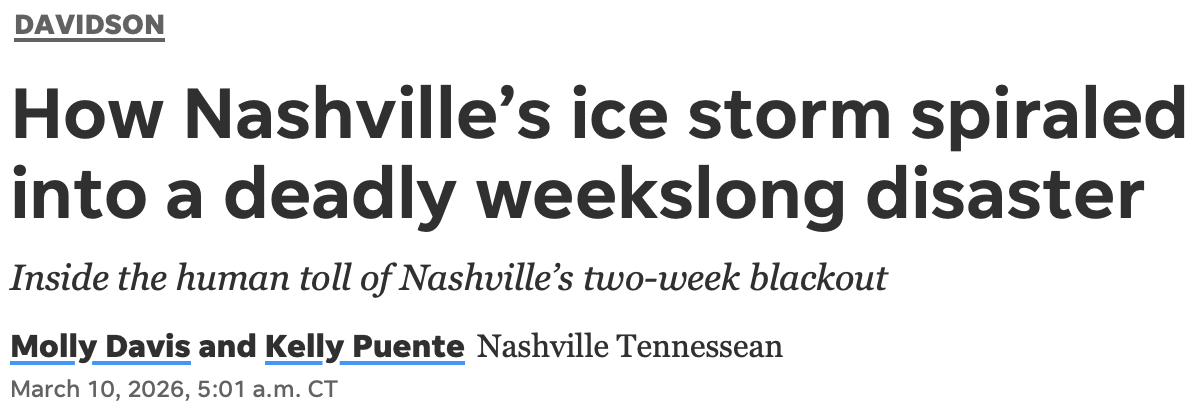
\includegraphics[width=0.8\linewidth]{headline.png}};
  % quotation marks are overlays, so they do not change the figure size
  \node[overlay, anchor=north east, inner sep=0pt, xshift=-12pt, yshift=12pt,
        font=\fontsize{160}{160}\selectfont\bfseries, text=utorange]
    at (img.north west) {``};
  \node[overlay, anchor=north west, inner sep=0pt, xshift=12pt, yshift=0.55in,
        font=\fontsize{160}{160}\selectfont\bfseries, text=utorange]
    at (img.south east) {''};
  \path[use as bounding box] ([yshift=0.15in]img.north west)
                             rectangle ([yshift=-0.1in]img.south east);
\end{tikzpicture}
\end{center}
\par
 \captionof{figure}{The \textit{Nashville Tennessean} on Winter Storm Fern~[1].}\par}
\vspace{\figgap}

We couple traffic, EV charging, weather, building, and power grid models to
study how cities respond to different scenarios, from extreme weather to new
infrastructure. Nashville serves as our first case study.

\subhead{Integrating models shows the full impact of a scenario}
Urban systems such as traffic, buildings, and the power grid depend on each
other, yet most models simulate only one of them. Coupling the models reveals
how a change in one system affects the others.

\subhead{Geospatial models need a new framework}
Our models exchange \textbf{geospatial entities}: real-world objects with a
location, a time, and properties, such as an EV. To our knowledge, no flexible
framework exists that exchanges such entities between models in a shared space
and time.
\end{posterbox}
\boxgap
\begin{posterbox}{Objectives}
\RaggedRight
\textbf{ORIGIN} (\textbf{O}ak \textbf{R}idge \textbf{I}ntegrated \textbf{G}rid,
\textbf{I}nfrastructure, and \textbf{N}etwork Model) has two goals:
\begin{enumerate}
  \item Develop ORIGIN as a flexible, fast, reusable, and spatial framework
  \item Demonstrate it with ORIGIN: Nashville, our first case study
\end{enumerate}
\end{posterbox}
\boxgap
\begin{posterbox}{Methods}
\RaggedRight
\topsubhead{ORIGIN: Flexible, fast, reusable, and spatial integration}
ORIGIN supports two kinds of models: \textbf{live models}, which it runs step
by step during the simulation, and \textbf{pre-run models}, which run
beforehand and whose results are loaded into the \textbf{State Memory},
ORIGIN's shared database.
\end{posterbox}
\end{minipage}%
\hspace{\posgap}%
% ========================= COLUMN 2 ===================================
\begin{minipage}[t]{\colwidth}\vspace{0pt}
\begin{posterbox}{Methods (continued)}
\RaggedRight
\subsubhead{Flexible}
The requirements on live models are minimal: the \textbf{Supervisory Model},
which coordinates all models, must be able to \textbf{write their inputs},
\textbf{advance them by one model timestep}, and \textbf{read their
outputs}. Models can run on one computer or spread across several.

\posterdiagram{figures/fig_lifecycle.tex}{Life cycle of a model in the ORIGIN
  framework. The Supervisory Model repeatedly calls steps 2--4 every model
  timestep until the simulation ends.}
\addvspace{\figgap}

\subsubhead{Fast setup}
A live model defines only four components: one or more \textbf{Outputs} and
\textbf{Inputs}, one \textbf{Adapter}, and one \textbf{ModelSpec}. A pre-run
model only defines its Outputs.

\subsubhead{Reusable}
The \textbf{Supervisory Model}, \textbf{Adapter Worker}, \textbf{Message
Broker}, and \textbf{State Memory} are model-agnostic: they work with any
model without changes.

\posterdiagram{figures/fig_architecture.tex}{Software architecture of the ORIGIN framework.}
\addvspace{\figgap}

\subsubhead{Spatial {\mdseries\itshape (in development)}}
The State Memory places all entities in a shared space and time and builds
each model's inputs from it.
\end{posterbox}
\end{minipage}%
\hspace{\posgap}%
% ========================= COLUMN 3 ===================================
\begin{minipage}[t]{\colwidth}\vspace{0pt}
\begin{posterbox}{Methods (continued)}
\RaggedRight
\topsubhead{ORIGIN: Nashville couples five urban models}
The models currently cover a test area in Nashville and will later cover all
of Davidson County, TN:
\begin{itemize}
  \item \textbf{Traffic:} SUMO (Simulation of Urban Mobility)
  \item \textbf{EV charging:} ORNL-developed model
  \item \textbf{Building:} AutoBEM (Automatic Building Energy Modeling)
  \item \textbf{Weather:} WRF (Weather Research and Forecasting)
  \item \textbf{Power grid:} ORNL-developed model
\end{itemize}
\end{posterbox}
\boxgap
\begin{posterbox}{Results (preliminary)}
\RaggedRight
We ran our first 24-hour scenario in the Nashville test area, showing that 
ORIGIN can couple models and exchange data between them. It tested the impact 
of new businesses: a corporate office, a data center, and a distribution facility.

\posterdiagram{figures/fig_framework.tex}{Model coupling in the new-business scenario.}
\end{posterbox}
\boxgap
\begin{posterbox}{Conclusion \& Future Work}
\RaggedRight
We built a first version of the flexible, fast, and reusable ORIGIN framework
and successfully ran it on a Nashville test area. Next, we will:
\begin{enumerate}
  \item Develop the framework further and finalize the State Memory's design
  \item Run more scenarios, including a 3-day heat wave and Winter Storm Fern
  \item Benchmark ORIGIN, possibly against other coupling approaches
\end{enumerate}

% GitHub card with QR code
\par\addvspace{\figgap}
\begin{tcolorbox}[enhanced, colback=utorange!8, colframe=utorange!60,
  boxrule=2pt, arc=0.2in, left=0.25in, right=0.25in, top=0.2in, bottom=0.2in,
  before skip=0pt, after skip=0pt]
\begin{minipage}[c]{2.4in}
  \qrcode[height=2.4in]{https://github.com/gaberm/origin-framework}
\end{minipage}\hspace{0.4in}%
\begin{minipage}[c]{\dimexpr\linewidth-2.8in\relax}
  {\fontsize{40}{48}\selectfont\bfseries Follow ORIGIN\par}
  \vspace{10pt}
  \githubmark[utsmokey]{0.4in}\hspace{0.12in}{\color{utsmokey}github.com/gaberm/origin-framework}
\end{minipage}
\end{tcolorbox}
\end{posterbox}
\boxgap
\begin{posterbox}{References}
\RaggedRight
{\fontsize{26}{32}\selectfont
\begin{enumerate}[label={[\arabic*]}, leftmargin=2em]
  \item M.~Davis and K.~Puente, ``How Nashville's ice storm spiraled into a
        deadly weekslong disaster,'' \textit{The Tennessean}, Mar.~10, 2026.
        Accessed: Oct.~14, 2026.
        \url{https://www.tennessean.com/story/news/local/davidson/2026/03/10/nashville-winter-storm-power-outage-timeline/88478822007/}
\end{enumerate}}
\end{posterbox}
\end{minipage}

% ========================= FOOTER: ACKNOWLEDGMENTS =====================
\par\vfill
{\centering\fontsize{22}{28}\selectfont\color{utsmokey}
This material is based upon work supported by the U.S. Department of Energy,
Office of Energy Efficiency and Renewable Energy, specifically the Energy Grid
Integration Office under contract number DE-AC05-00OR22725. The views expressed
herein do not necessarily represent the views of the U.S. Department of Energy
or the United States Government.\par}

\end{document}
